\section{Controller PID}
\label{PID}

\begin{figure}[htb]
\centering
\label{PIDimage}
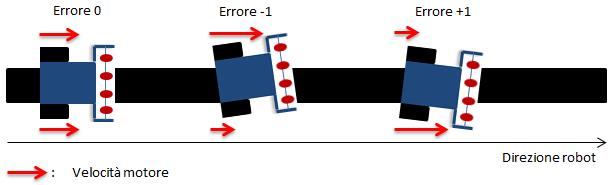
\includegraphics[width=0.65 \textwidth]{PID.jpg} 
\caption{prova}
\end{figure}

\begin{figure}[htb]
\centering
\label{PD}
\begin{tikzpicture}[->, >=stealth', shorten >=0.1pt, auto, node distance=2cm, semithick,
								  hv path/.style={to path={-| (\tikztotarget)}},
								  tip/.style={->,shorten >=0.007pt}, 
								  vh path/.style={to path={|- (\tikztotarget)}}]

%====Definizione stile stati===============================================

	\tikzstyle{sommatore} = [circle, draw, text centered,  minimum width =0.02cm]
  	\tikzstyle{block}			=	[rectangle, draw, text centered, minimum height =1cm]
  	\tikzstyle{line} = [, draw]
%====Definizione stati e posizione==========================================
	\node[] 					(A) [label = set point]                   		{};
	\node[sommatore]  (B) [right of=A, node distance = 3cm, label = -240:$+$,label = -120:$-$]		{$\sum$};			
	\node[block]			(C) [right of=B, node distance = 3cm ]		{\textsc{pd}};
  	\node[sommatore] 	(D) [right of=C,node distance = 	3cm 	]		{} ;
  	\node[]         			(E) [right of=D,node distance = 	3cm, label = 90:uscita, label =- 90: velocita motori]  		{};
 	\node[]         			(F) [below of=B]  	{};
  	\node[]         			(G) [below of=D]  	{};
  	\node[block]         	(H) [below of=C]  	{\textsc{sensori di linea}}; 	
%====Definizione chain==================================================
    
       \path	 	(A) edge (B)
        			 	(B) edge node{errore}(C)
        				(C) edge (D);
        { [start chain]
        \chainin	(D) [join];
        { [start branch=minus]
        	\chainin (H) [join=by {vh path,tip}];
        	\chainin (B) [join=by {hv path,tip}];
        }
		\chainin(E) [join];				
    }				
\end{tikzpicture}
\caption{prova}
\end{figure}
